\documentclass[12]{article}
\usepackage[utf8]{inputenc}
\usepackage{algorithmic}
\usepackage{tikz}
\documentclass[runningheads]{llncs}
\usepackage{graphicx}
\usepackage{listings}
\usepackage{pgfplots}
\usepackage{algorithm}
\usepackage[noend]{algpseudocode}
\usepackage{float}
\usepackage[section]{placeins}

\title{QuizzGame}
\author{Martisca Filip }
\date{Decembrie 2020}

\begin{document}

\maketitle

\section{Introducere}
\hspace{5mm} In acest raport vom prezenta caracteristicile si implementarea aplicatiei QuizzGame. QuizzGame este o aplicatie in care clientul primeste intrebari de la server avand un anumit timp pentru a raspunde, ulterior clientul va fi evaluat in functie de raspunsurile lui va primi o nota.
\State
\hspace{5mm} Intrebarile vor fi trimise in ordinea inregistrarii utilizatorilor iar cand ultimul utilizator inregistrat va termina de raspuns la intrebari toti utilizatorii vor primi un mesaj cu utilizatorul care a avut scorul cel mai mare.

\section{Tehnologii utilizate}
\hspace{5mm} In realizarea conexiunii dintre server si client am folosit modelul TCP. Am folosit modelul TCP care este orientat-conexiune deoarece avem siguranta ca datele noastre vor ajunge intacte si in ordinea in care le-am trimis. Atunci cand un client se va deconecta ceilalti participanti pot continua raspunde la intrebari.  
\State \hspace{5mm} Serverul nostru va fi multithreading (va crea cate un thread pentru fiecare client) deci fiecare client va comunica independent cu serverul. Threadurile ultilizeaza mai putine resurse decat procesele iar comuncarea intre threaduri se poate face mai usor.

\section{Arhitectura aplicatiei}
\hspace{5mm}Toti userii, intrebarile si raspunsurile vor fi stocate intr o baza de date SqLite in care vom avea mai multe tabele: user, question, answer ...  

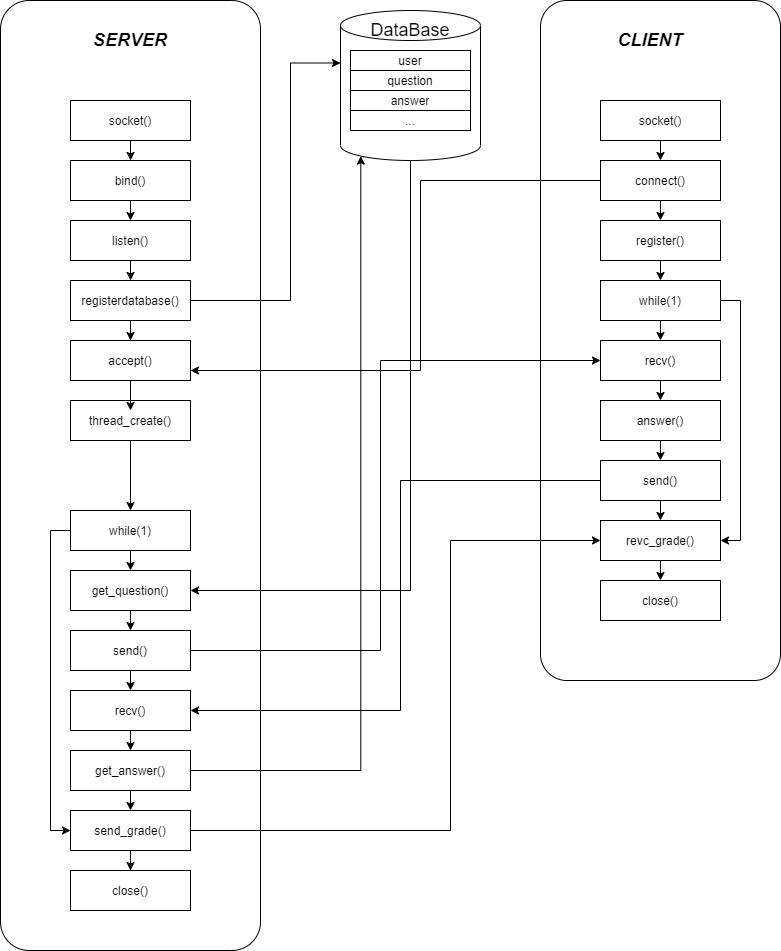
\includegraphics[scale=0.41]{serverclient.png}

\section{Detalii implementare}
\hspace{5mm}Atunci cand clientul realizeaza conexiunea cu serverul trebuie sa se inregistreze cu un username si cu un email, care apoi este trimis la server iar acesta le memoreaza intr-o baza de date impreuna cu un id unic. 
\State \hspace{5mm}In server se va selecta o intrebare cu variante de raspuns din baza de date care va fi trimisa clientului. Intr-un numar de secunde stabilit clientul trebuie sa raspunda la intrebare, in caz contrar va primi 0 puncte(dupa ce trece timpul apare automat urmatoarea intrebare). Se trimite raspunsul la server iar acesta ii calculeaza punctajul.
\State
\State \hspace{5mm} Cand se epuizeaza setul de intrebari clientii vor primi punctajul iar dupa ce au terminat toti clientii se va trimite tuturor un mesaj cu numele clientului care a castigat.
\State \hspace{5mm} Clientul poate iesi oricand din joc trimitand "exit" ca raspuns la orice intrebare. 
\State
\State
\State
\begin{lstlisting}[]
//primire raspuns/intrebare
    bzero(buf, sizeof(buf));
if (read (sd, &buf,sizeof(buf)) < 0) 
    {
      perror ("[client]Eroare la read() de la server.\n");
      return errno;
    }
    cout<<buf<<endl;
}
\end{lstlisting}

\State
\begin{lstlisting}[]
//trimitere raspuns
printf ("[client]Introduceti un raspuns: "); 
  fflush (stdout);
  bzero(buf, sizeof(buf));
  scanf("%s",buf);
 
  if (write (sd,&buf,sizeof(buf)) <= 0)
    {
      perror ("[client]Eroare la write() spre server.\n");
      return errno;
    }

\end{lstlisting}
\State
\begin{lstlisting}[]
\\selectare id pentru crearea unui nou id
while((rc=sqlite3_step(stmt))==SQLITE_ROW)
       {
           sent= sqlite3_column_int(stmt,0);
       }
       sqlite3_finalize(stmt);
       return sent;
\end{lstlisting}

\section{Concluzii}
\hspace{5mm}Aceasta aplicatie poate avea ca scop evaluarea unor persoane (test) dar poate sa fie si un joc de cultura generala pe care il poti juca cu prietenii.
\State \hspace{5mm} O varianta mai buna in materie  de timp ar fi utilizarea modelului TCP cu select() si I/O neblocante in loc de TCP multithreading. 
\State \hspace{5mm}O imbunatatire semnificativa a aplicatiei ar fi realizarea unei interfete deoarece va fi mult mai interactiva si mai placuta de client. O alta imbunatatire ar fi adaugarea unui timer pentru a vedea timpul ramas. 


\begin{thebibliography}{9}

\bibitem{}
  \url{https://profs.info.uaic.ro/~computernetworks/cursullaboratorul.php}
  
 \bibitem{}
 \url{https://en.wikipedia.org/wiki/Transmission\_Control\_Protocol}
 
  \bibitem{}
 \url{https://www.backblaze.com/blog/whats-the-diff-programs-processes-and-threads/}
 
 \bibitem{}
  \url{https://stackoverflow.com/questions/3756882/detached-vs-joinable-posix-threads}
  
   \bibitem{}
  \url{https://www.geeksforgeeks.org/sql-using-c-c-and-sqlite/?ref=rp}
  
  \bibitem{}
  \url{https://stackoverflow.com/questions/263116/c-waiting-for-all-threads-to-complete}
  
 \bibitem{}
  \url{https://www.youtube.com/watch?v=It0OFCbbTJE&ab\_channel=JacobSorber}
  
  \bibitem{}
  \url{https://computing.llnl.gov/tutorials/pthreads/}
  
  \bibitem{}
  \url{https://www.sqlite.org/index.html}
  
  
 \bibitem{}
  \url{https://www.geeksforgeeks.org/tcp-3-way-handshake-process/?ref=rp}
  
  
  
\end{thebibliography}  
\end{document}
